\documentclass[
11pt, % The default document font size, options: 10pt, 11pt, 12pt
%codirector, % Uncomment to add a codirector to the title page
]{charter} 




% El títulos de la memoria, se usa en la carátula y se puede usar el cualquier lugar del documento con el comando \ttitle
\titulo{Sensor de Estacionamiento LoRaWAN} 

% Nombre del posgrado, se usa en la carátula y se puede usar el cualquier lugar del documento con el comando \degreename
\posgrado{Carrera de Especialización en Sistemas Embebidos} 
%\posgrado{Carrera de Especialización en Internet de las Cosas} 
%\posgrado{Carrera de Especialización en Intelegencia Artificial}
%\posgrado{Maestría en Sistemas Embebidos} 
%\posgrado{Maestría en Internet de las cosas}

% Tu nombre, se puede usar el cualquier lugar del documento con el comando \authorname
\autor{Ing. Cristian Funes} 

% El nombre del director y co-director, se puede usar el cualquier lugar del documento con el comando \supname y \cosupname y \pertesupname y \pertecosupname
\director{Ing. Ernesto Chediack}
\pertenenciaDirector{CEGA Electrónica}
%\codirector{John Doe} % para que aparezca en la portada se debe descomentar la opción codirector en el documentclass
%\pertenenciaCoDirector{FIUBA}

% Nombre del cliente, quien va a aprobar los resultados del proyecto, se puede usar con el comando \clientename y \empclientename
\cliente{Ernesto Chediack}
\empresaCliente{CEGA Electrónica}

% Nombre y pertenencia de los jurados, se pueden usar el cualquier lugar del documento con el comando \jurunoname, \jurdosname y \jurtresname y \perteunoname, \pertedosname y \pertetresname.
\juradoUno{Nombre y Apellido (1)}
\pertenenciaJurUno{pertenencia (1)} 
\juradoDos{Nombre y Apellido (2)}
\pertenenciaJurDos{pertenencia (2)}
\juradoTres{Nombre y Apellido (3)}
\pertenenciaJurTres{pertenencia (3)}
 
\fechaINICIO{20 de octubre de 2022}		%Fecha de inicio de la cursada de GdP \fechaInicioName
\fechaFINALPlan{8 de diciembre de 2022} 	%Fecha de final de cursada de GdP
\fechaFINALTrabajo{20 de octubre de 2023}	%Fecha de defensa pública del trabajo final


\begin{document}

\maketitle
\thispagestyle{empty}
\pagebreak


\thispagestyle{empty}
{\setlength{\parskip}{0pt}
\tableofcontents{}
}
\pagebreak


\section*{Registros de cambios}
\label{sec:registro}


\begin{table}[ht]
\label{tab:registro}
\centering
\begin{tabularx}{\linewidth}{@{}|c|X|c|@{}}
\hline
\rowcolor[HTML]{C0C0C0} 
Revisión & \multicolumn{1}{c|}{\cellcolor[HTML]{C0C0C0}Detalles de los cambios realizados} & Fecha      \\ \hline
0      & Creación del documento                                 &\fechaInicioName \\ \hline
1      & Se completa hasta el punto 5 inclusive                 & 03/11/2022 \\ \hline
2      & Se completa hasta el punto 9 inclusive	                & 10/11/2022 \\ \hline
%3      & Se completa hasta el punto 11 inclusive                & dd/mm/aaaa \\ \hline
%4      & Se completa el plan	                                 & dd/mm/aaaa \\ \hline
\end{tabularx}
\end{table}

\pagebreak



\section*{Acta de constitución del proyecto}
\label{sec:acta}

\begin{flushright}
Buenos Aires, \fechaInicioName
\end{flushright}

\vspace{2cm}

Por medio de la presente se acuerda con el Ing. \authorname\hspace{1px} que su Trabajo Final de la \degreename\hspace{1px} se titulará ``\ttitle'', consistirá esencialmente en la implementación de un prototipo de un sensor de estacionamiento con conectividad LoRaWAN, y tendrá un presupuesto preliminar estimado de 600 hs de trabajo y \$500000, con fecha de inicio \fechaInicioName\hspace{1px} y fecha de presentación pública \fechaFinalName.

Se adjunta a esta acta la planificación inicial.

\vfill

% Esta parte se construye sola con la información que hayan cargado en el preámbulo del documento y no debe modificarla
\begin{table}[ht]
\centering
\begin{tabular}{ccc}
\begin{tabular}[c]{@{}c@{}}Ariel Lutenberg \\ Director posgrado FIUBA\end{tabular} & \hspace{2cm} & \begin{tabular}[c]{@{}c@{}}\clientename \\ \empclientename \end{tabular} \vspace{2.5cm} \\ 
\multicolumn{3}{c}{\begin{tabular}[c]{@{}c@{}} \supname \\ Director del Trabajo Final\end{tabular}} \vspace{2.5cm} \\
%\begin{tabular}[c]{@{}c@{}}\jurunoname \\ Jurado del Trabajo Final\end{tabular}     &  & \begin{tabular}[c]{@{}c@{}}\jurdosname\\ Jurado del Trabajo Final\end{tabular}  \vspace{2.5cm}  \\
%\multicolumn{3}{c}{\begin{tabular}[c]{@{}c@{}} \jurtresname\\ Jurado del Trabajo Final\end{tabular}} \vspace{.5cm}                                                                     
\end{tabular}
\end{table}




\section{1. Descripción técnica-conceptual del proyecto a realizar}
\label{sec:descripcion}

El proyecto que aquí se describe consiste en la implementación de un sensor de estacionamiento con conectividad LoRaWAN. El sensor será del tipo "tacha", como puede verse en la Figura \ref{fig:ParkingSensor}.

\vspace{25px}

\begin{figure}[H]
\centering 
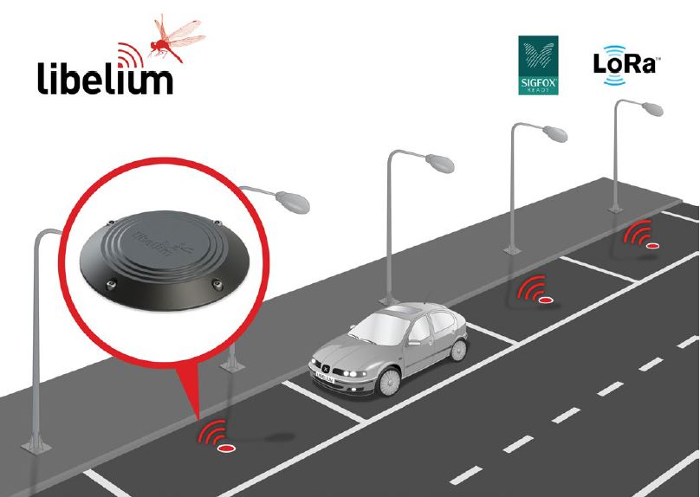
\includegraphics[width=.75\textwidth]{./Figuras/ParkingSensor.jpg}
\caption{Sensor de estacionamiento.}
\label{fig:ParkingSensor}
\end{figure}

\vspace{25px}

El objetivo es poder aplicar este tipo de dispositivos a soluciones de Smart Parking.\\
Cuando el sensor detecte que un vehículo se encuentra posicionado por encima, enviará un mensaje a un servidor LoRaWAN a través de un Gateway LoRa para dar aviso de dicho evento. Lo mismo ocurrirá cuando se detecte que el vehículo se ha retirado. Esta información permitirá conocer cuánto tiempo estuvo un vehículo estacionado. Además, sabiendo la ubicación de cada sensor de estacionamiento, será posible visualizar en tiempo real los espacios ocupados y disponibles para estacionar.\\
En la Figura \ref{fig:ParkingSensorDiagram} puede verse un diagrama en bloques del sistema propuesto:

\vspace{25px}

\begin{figure}[H]
\centering 
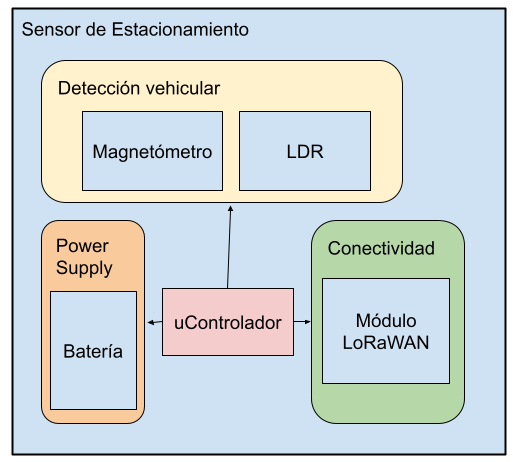
\includegraphics[width=.75\textwidth]{./Figuras/DiagramaBloqueSensor.png}
\caption{Diagrama en bloques del sensor de estacionamiento.}
\label{fig:ParkingSensorDiagram}
\end{figure}

\vspace{25px}

Se observa que el equipo se alimenta a baterías. Esto es un desafío ya que debe lograrse una autonomía de al menos un año para que el proyecto sea escalable.\\
Como método de detección se empleará un conjunto magnetómetro-LDR. La idea es poder evitar falsas detecciones usando ambos sensores. Cuando un vehículo se posicione arriba del sensor, se producirá una variación en la intensidad luminosa que será medida por el LDR. Esto, en junto con la variación de campo magnético producida por la masa vehicular, permitirá mejorar la exactitud de las detecciones, evitando falsos positivos y falsos negativos.\\
El microcontrolador será el encargado de realizar la lectura de los sensores, como también de controlar la comunicación LoRaWAN y el consumo de energía.


\section{2. Identificación y análisis de los interesados}
\label{sec:interesados}


\begin{table}[ht]
%\caption{Identificación de los interesados}
%\label{tab:interesados}
\begin{tabularx}{\linewidth}{@{}|l|X|X|l|@{}}
\hline
\rowcolor[HTML]{C0C0C0} 
Rol           & Nombre y Apellido & Organización 	& Puesto 	\\ \hline
Auspiciante   & Ernesto Chediack  & CEGA Electronica& Gerente de Ingenieria \\ \hline
Cliente       & \clientename      &\empclientename	& Gerente de Ingenieria
\\ \hline
Responsable   & \authorname       & FIUBA        	& Alumno 	\\ \hline
Colaboradores & Gabriel Caballero & CEGA Electrónica& Desarrollador\\ \hline
Orientador    & \supname	      & \pertesupname 	& Director Trabajo final \\ \hline
Equipo        & José Bosdari      & Supercanal     	& Gerente I+D\\ \hline
Usuario final & -                 & Municipalidad de Luján de Cuyo& -       	\\ \hline
\end{tabularx}
\end{table}



\section{3. Propósito del proyecto}
\label{sec:proposito}

El propósito de este proyecto es desarrollar un sensor de estacionamiento que pueda ser utilizado en aplicaciones de Smart Parking. Para ello debe ser fácilmente escalable y contar con suficiente autonomía energética.


\section{4. Alcance del proyecto}
\label{sec:alcance}

El presente proyecto incluye:
\begin{itemize}
	\item Diseño, implementación y montaje de una placa funcional para el sensor de estacionamiento.
	\item Desarrollo del firmware para el microcontrolador del sensor de estacionamiento.
	\item Desarrollo del entorno de testing.
	\item Puesta en marcha de una red de 10 sensores para la Municipalidad de Luján de Cuyo.
\end{itemize}

El presente proyecto no incluye:
\begin{itemize}
	\item Despliegue de red de mas de 10 sensores.
	\item Configuración de Gateway LoRaWAN.
	\item Diseño de gabinete.
	\item Desarrollo de aplicación de parquímetro.
\end{itemize}

\section{5. Supuestos del proyecto}
\label{sec:supuestos}

Para el desarrollo del siguiente proyecto se supone que:
\begin{itemize}
	\item Se conseguirán todos los componentes necesarios para la implementación del dispositivo.
	\item Se podrá acceder a una red LoRa.
	\item Se podrá utilizar la banda ISM 915MHz.
	\item Se podrán realizar las pruebas y mediciones necesarias para calcular la autonomía del dispositivo.
	\item El auspiciante mantendrá el interés en continuar con el desarrollo del proyecto durante toda la duración del mismo.
\end{itemize}


\section{6. Requerimientos}
\label{sec:requerimientos}

A continuación se enumeran los requerimientos del proyecto. Se han agrupado de acuerdo a su afinidad en requerimientos funcionales, no funcionales, de la interfaz externa, de diseño del hardware, de testing, de documentación y opcionales. Se le asigna a cada requerimiento un nivel de prioridad del 1 al 5, siendo 1 la prioridad más alta y 5 la prioridad más baja.

\begin{enumerate}
	\item Requerimientos funcionales
		\begin{enumerate}
			\item El equipo debe detectar vehículos utilizando un LDR y un magnetómetro [1].
			\item El equipo debe conectarse a una red LoRaWAN [1].
			\item El equipo debe enviar un mensaje cada vez que cambie el estado de detección de un vehículo [1].
			\item El equipo debe auto calibrarse cuando se lo encienda por primera vez, para configurar un umbral de detección de vehículos [1].
			\item El equipo debe reportar el nivel de batería cada vez que envía un mensaje por la red LoRaWAN [2].
			\item El equipo debe salir configurado de fábrica con todas las claves necesarias para conectarse a un servidor LoRaWAN [2].
			\item El equipo debe tener un modo de trabajo offline, donde se pueda guardar cada evento hasta que se recupere la conexión con la red LoRaWAN [3].
			\item El equipo debe enviar un mensaje de keep alive cada 12 horas por la red LoRaWAN [3].
			\item El equipo debe reportar que se detectó o se dejó de detectar un vehículo dentro de los 2 minutos de producido el evento [3].
		\end{enumerate}
	\item Requerimientos no funcionales
		\begin{enumerate}
			\item El equipo debe operar en la banda de uso compartido sin autorización comprendida entre 915 MHz y 928 MHz [1].
			\item Todo el firmware desarrollado para el proyecto deberá estar correctamente versionado  usando una herramienta de control de versiones [1].
			\item Se deberán realizar revisiones de código con los miembros del equipo de trabajo cuando se integren nuevas funcionalidades el firmware [2].
			\item Cada equipo deberá contar con un número de serie que permita la trazabilidad y la localización geográfica del mismo [2].
			\item Se deberán liberar releases de firmware intermedias al cliente para analizar el estado de avance del proyecto [3].
			\item Se deberá programar reuniones mensuales con el cliente para analizar el estado del proyecto [3].
		\end{enumerate}
	\item Requerimientos de la interfaz externa
		\begin{enumerate}
			\item El equipo debe montarse dentro de una tacha reductora de velocidad [1].
		\end{enumerate}
	\item Requerimientos de diseño del hardware
		\begin{enumerate}
			\item El equipo debe alimentarse con baterías [1].
			\item El desarrollo deberá realizarse utilizando un microcontrolador [1].
			\item El equipo debe incluir un módulo de comunicaciones LoRa [1].
			\item El equipo debe tener una autonomía de por lo menos 1 año [3].
		\end{enumerate}
	\item Requerimientos de testing
		\begin{enumerate}
			\item Cada módulo de software implementado debe contar con un coverage de código mayor al 80\% [2].
			\item El entorno de desarrollo de software debe contar con la posibilidad de ejecutar tests unitarios automáticamente cuando se suba código nuevo al repositorio [3].
			\item Deben realizarse tests de integración [5].
			\item Deben realizarse tests del tipo end to end [5].
		\end{enumerate}
	\item Requerimientos de documentación
		\begin{enumerate}
			\item Se deberá redactar una memoria técnica del proyecto según la fecha definida en este documento [1].
			\item Se deberá documentar el software desarrollado utilizando doxygen [2].
			\item Se deberá entregar un manual que detalle el correcto uso del equipo [3].
		\end{enumerate}
	\item Requerimientos opcionales
		\begin{enumerate}
			\item El equipo debe ser capaz de recibir mensajes de configuración a través de la red LoRaWAN [5].
		\end{enumerate}
\end{enumerate}
 


\section{7. Historias de usuarios (\textit{Product backlog})}
\label{sec:backlog}

En esta sección se detallan las historias de usuario. Las mismas se desarrollaron desde el punto de vista del cliente. Los story points se calcularon como la suma de cada uno de los distintos aspectos que se detallan a continuación:
\begin{enumerate}
	\item La \textit{prioridad} es el interés del cliente por incluir una característica. Se divide en distintos valores a los cuales se les asigna un peso numérico:
		\begin{enumerate}
	 		\item Alta [5].
	 		\item Media [3].
	 		\item Baja [2].
	 		\item Muy baja [1].
	 	\end{enumerate} 
	 \item La \textit{cantidad de trabajo} es una medida del esfuerzo asociado para desarrollar la tarea:
	 	\begin{enumerate}
	 		\item Alta [8].
	 		\item Media [5].
	 		\item Baja [3].
	 	\end{enumerate}
	 \item La \textit{complejidad} es una medida de lo difícil que se espera que sea implementar la característica:
	 	\begin{enumerate}
	 		\item Alta [13].
	 		\item Media [8].
	 		\item Baja [5].
	 	\end{enumerate}
	 \item El \textit{riesgo e incertidumbre} es una medida del impacto que tiene implementar la característica:
	 	\begin{enumerate}
	 		\item Alta [8].
	 		\item Media [3].
	 		\item Baja [1].
	 	\end{enumerate}
\end{enumerate}

\begin{enumerate}
\item \textit{Historia de usuario 1.} El cliente quiere instalar el equipo en la calle sin tener que realizar conexiones de ningún tipo, para poder reducir el tiempo de instalación y el costo de mantenimiento.
	\begin{itemize}
		\item Prioridad: Alta.
		\item Cantidad de trabajo: Media .
		\item Complejidad: Media.
		\item Riesgo e incertidumbre: Baja.
		\item Story points: 19.
	\end{itemize}
	
	\item \textit{Historia de usuario 2.} El cliente quiere conectar miles de sensores de estacionamiento dentro de la misma red para poder reducir los costos de mantenimiento.
	\begin{itemize}
		\item Prioridad: Media.
		\item Cantidad de trabajo: Baja.
		\item Complejidad: Media.
		\item Riesgo e incertidumbre: Alta.
		\item Story points: 22.
	\end{itemize}
	
		\item \textit{Historia de usuario 3.} El cliente quiere poder conocer en tiempo real el estado de cada uno de los sensores, para poder determinar el tiempo que un vehículo se encuentra estacionado.
	\begin{itemize}
		\item Prioridad: Alta.
		\item Cantidad de trabajo: Baja.
		\item Complejidad: Baja.
		\item Riesgo e incertidumbre: Baja.
		\item Story points: 14.
	\end{itemize}
	
	\item \textit{Historia de usuario 4.} El cliente quiere poder conocer la ubicación geográfica de cada uno de los sensores, para poder determinar qué espacios están disponibles para estacionar.
	\begin{itemize}
		\item Prioridad: Alta.
		\item Cantidad de trabajo: Baja.
		\item Complejidad: Baja.
		\item Riesgo e incertidumbre: Media.
		\item Story points: 16.
	\end{itemize}
	
	\item \textit{Historia de usuario 5.} El cliente quiere que la red de sensores use una banda de frecuencias del espectro de RF no licenciado, para reducir los costos de operación.
	\begin{itemize}
		\item Prioridad: Muy baja.
		\item Cantidad de trabajo: Baja.
		\item Complejidad: Media.
		\item Riesgo e incertidumbre: Alta.
		\item Story points: 20.
	\end{itemize}
\end{enumerate}

\section{8. Entregables principales del proyecto}
\label{sec:entregables}

Los entregables del proyecto son:
	\begin{enumerate}
		\item Manual de usuario.
		\item Prototipo funcional.
		\item Diagramas de circuitos.
		\item Código fuente del firmware.
		\item Informe final.
	\end{enumerate}

\section{9. Desglose del trabajo en tareas}
\label{sec:wbs}

A continuación se detalla el desglose de tareas, con un detalle de las horas que se estima llevará finalizar cada una:
	\begin{enumerate}
		\item Organización del proyecto (50hs)
			\begin{enumerate}
				\item Configuración de las herramientas para gestión (5hs). 
				\item Elaboración del informe de planificación del proyecto (40hs).
				\item Ajuste y control de avance de las tareas (5hs).
			\end{enumerate}
		\item Investigación preliminar (32hs)
			\begin{enumerate}
				\item Investigación sobre productos similares en el mercado (8hs).
				\item Investigación sobre redes LoRaWAN (16hs).
				\item Investigación sobre sistemas de detección basados en magnetómetro (8hs).
			\end{enumerate}
		\item Investigación de hardware (30hs)
			\begin{enumerate}
				\item Investigación y selección de módulo LoRaWAN (6hs).
				\item Investigación y selección de magnetómetro (6hs).
				\item Investigación y selección de microcontrolador (4hs).
				\item Investigación y selección de baterías (8hs).
				\item Investigación y selección de reguladores de tensión para aplicaciones de bajo consumo energético (6hs).
			\end{enumerate}
		\item Desarrollo de hardware (156hs)
			\begin{enumerate}
				\item Desarrollo de circuito esquemático (40hs).
				\item Desarrollo de lista de materiales (4hs).
				\item Búsqueda y adquisición de componentes (6hs).
				\item Desarrollo de bibliotecas de componentes (16hs).
				\item Routeo del PCB (40hs).
				\item Enviar a fabricar PCB (2hs).
				\item Montaje del PCB (8hs).
				\item Pruebas de funcionamiento (16hs).
				\item Rediseño del PCB ante fallas (24hs).
			\end{enumerate}
		\item Investigación de firmware (16hs)
			\begin{enumerate}
				\item Investigación y selección de RTOS (8hs).
				\item Investigación sobre metodologías de trabajo (8hs).
			\end{enumerate}
		\item Desarrollo de firmware (368hs)
			\begin{enumerate}
				\item Creación de repositorios de trabajo (8hs).
				\item Instalación de las herramientas de trabajo (8hs).
				\item Diseño de la arquitectura de software (24hs).
				\item Selección y configuración de framework de testing (8hs).
				\item Desarrollo de los drivers para el magnetómetro (40hs).
				\item Desarrollo de los drivers para el módulo LoRaWAN (40hs).
				\item Desarrollo de las tareas de aplicación (120hs).
				\item Integración de los componentes de software (120hs).
			\end{enumerate}
		\item Integración (48hs)
			\begin{enumerate}
				\item Montaje del hardware en gabinete (8hs).
				\item Pruebas de campo (40hs).
			\end{enumerate}
		\item Documentación (72hs)
			\begin{enumerate}
				\item Generar manual de usuario (8hs).
				\item Generar documentación del firmware (8hs).
				\item Elaboración del informe final (40hs).
				\item Elaboración de la presentación final (16hs).
			\end{enumerate}
	\end{enumerate}

Cantidad total de horas: 772hs.

\section{10. Diagrama de Activity On Node}
\label{sec:AoN}

\begin{consigna}{red}
Armar el AoN a partir del WBS definido en la etapa anterior. 

%La figura \ref{fig:AoN} fue elaborada con el paquete latex tikz y pueden consultar la siguiente referencia \textit{online}:

%\url{https://www.overleaf.com/learn/latex/LaTeX_Graphics_using_TikZ:_A_Tutorial_for_Beginners_(Part_3)\%E2\%80\%94Creating_Flowcharts}

\end{consigna}

\begin{figure}[htpb]
\centering 
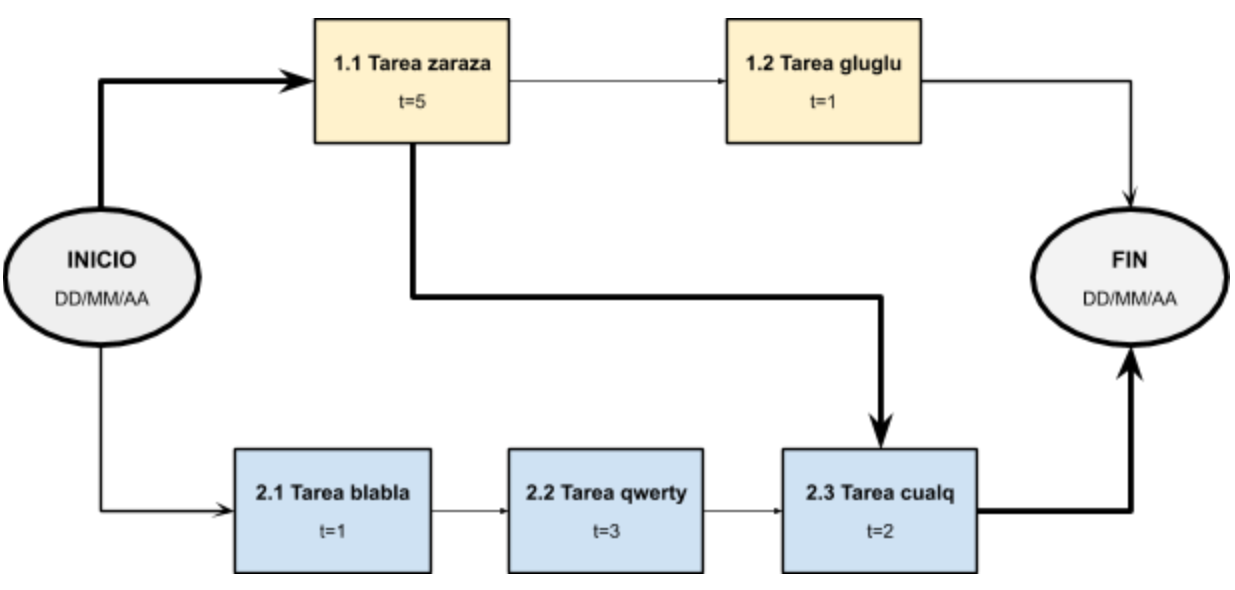
\includegraphics[width=.8\textwidth]{./Figuras/AoN.png}
\caption{Diagrama en \textit{Activity on Node}}
\label{fig:AoN}
\end{figure}

Indicar claramente en qué unidades están expresados los tiempos.
De ser necesario indicar los caminos semicríticos y analizar sus tiempos mediante un cuadro.
Es recomendable usar colores y un cuadro indicativo describiendo qué representa cada color, como se muestra en el siguiente ejemplo:



\section{11. Diagrama de Gantt}
\label{sec:gantt}

\begin{consigna}{red}

Existen muchos programas y recursos \textit{online} para hacer diagramas de gantt, entre los cuales destacamos:

\begin{itemize}
\item Planner
\item GanttProject
\item Trello + \textit{plugins}. En el siguiente link hay un tutorial oficial: \\ \url{https://blog.trello.com/es/diagrama-de-gantt-de-un-proyecto}
\item Creately, herramienta online colaborativa. \\\url{https://creately.com/diagram/example/ieb3p3ml/LaTeX}
\item Se puede hacer en latex con el paquete \textit{pgfgantt}\\ \url{http://ctan.dcc.uchile.cl/graphics/pgf/contrib/pgfgantt/pgfgantt.pdf}
\end{itemize}

Pegar acá una captura de pantalla del diagrama de Gantt, cuidando que la letra sea suficientemente grande como para ser legible. 
Si el diagrama queda demasiado ancho, se puede pegar primero la ``tabla'' del Gantt y luego pegar la parte del diagrama de barras del diagrama de Gantt.

Configurar el software para que en la parte de la tabla muestre los códigos del EDT (WBS).\\
Configurar el software para que al lado de cada barra muestre el nombre de cada tarea.\\
Revisar que la fecha de finalización coincida con lo indicado en el Acta Constitutiva.

En la figura \ref{fig:gantt}, se muestra un ejemplo de diagrama de gantt realizado con el paquete de \textit{pgfgantt}. En la plantilla pueden ver el código que lo genera y usarlo de base para construir el propio.

\begin{figure}[htbp]
\begin{center}
\begin{ganttchart}{1}{12}
  \gantttitle{2020}{12} \\
  \gantttitlelist{1,...,12}{1} \\
  \ganttgroup{Group 1}{1}{7} \\
  \ganttbar{Task 1}{1}{2} \\
  \ganttlinkedbar{Task 2}{3}{7} \ganttnewline
  \ganttmilestone{Milestone o hito}{7} \ganttnewline
  \ganttbar{Final Task}{8}{12}
  \ganttlink{elem2}{elem3}
  \ganttlink{elem3}{elem4}
\end{ganttchart}
\end{center}
\caption{Diagrama de gantt de ejemplo}
\label{fig:gantt}
\end{figure}


\begin{landscape}
\begin{figure}[htpb]
\centering 
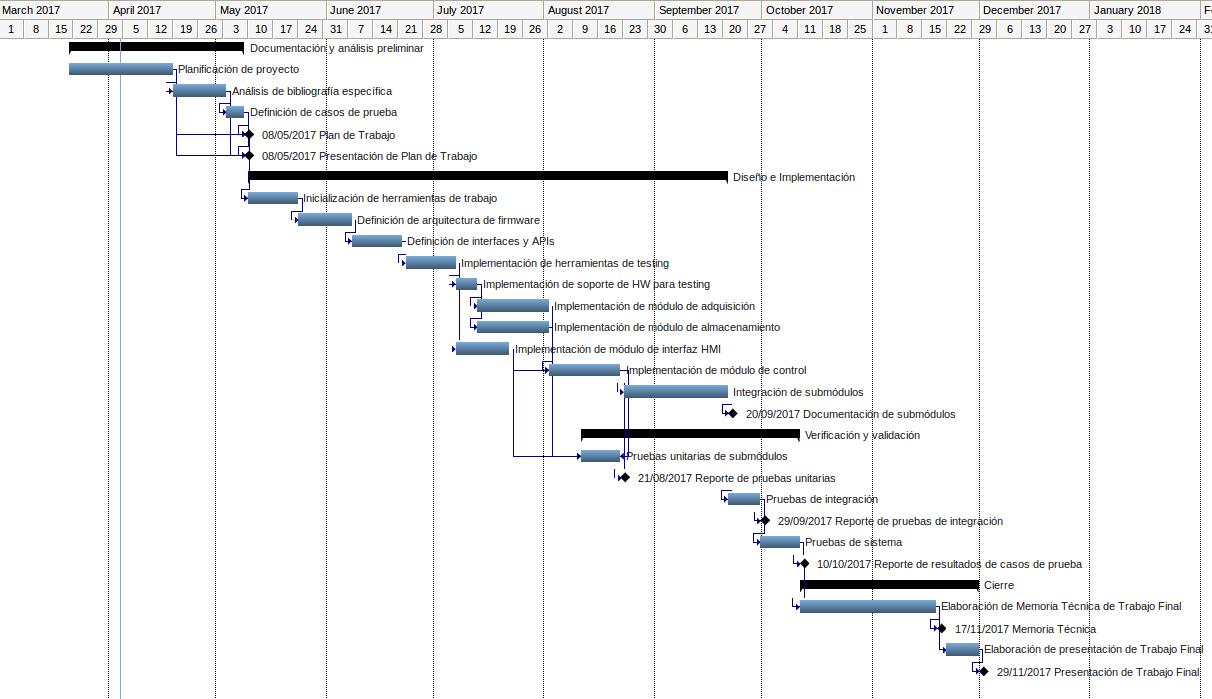
\includegraphics[height=.85\textheight]{./Figuras/Gantt-2.png}
\caption{Ejemplo de diagrama de Gantt rotado}
\label{fig:diagGantt}
\end{figure}

\end{landscape}

\end{consigna}


\section{12. Presupuesto detallado del proyecto}
\label{sec:presupuesto}

\begin{consigna}{red}
Si el proyecto es complejo entonces separarlo en partes:
\begin{itemize}
	\item Un total global, indicando el subtotal acumulado por cada una de las áreas.
	\item El desglose detallado del subtotal de cada una de las áreas.
\end{itemize}

IMPORTANTE: No olvidarse de considerar los COSTOS INDIRECTOS.

\end{consigna}

\begin{table}[htpb]
\centering
\begin{tabularx}{\linewidth}{@{}|X|c|r|r|@{}}
\hline
\rowcolor[HTML]{C0C0C0} 
\multicolumn{4}{|c|}{\cellcolor[HTML]{C0C0C0}COSTOS DIRECTOS} \\ \hline
\rowcolor[HTML]{C0C0C0} 
Descripción &
  \multicolumn{1}{c|}{\cellcolor[HTML]{C0C0C0}Cantidad} &
  \multicolumn{1}{c|}{\cellcolor[HTML]{C0C0C0}Valor unitario} &
  \multicolumn{1}{c|}{\cellcolor[HTML]{C0C0C0}Valor total} \\ \hline
 &
  \multicolumn{1}{c|}{} &
  \multicolumn{1}{c|}{} &
  \multicolumn{1}{c|}{} \\ \hline
 &
  \multicolumn{1}{c|}{} &
  \multicolumn{1}{c|}{} &
  \multicolumn{1}{c|}{} \\ \hline
\multicolumn{1}{|l|}{} &
   &
   &
   \\ \hline
\multicolumn{1}{|l|}{} &
   &
   &
   \\ \hline
\multicolumn{3}{|c|}{SUBTOTAL} &
  \multicolumn{1}{c|}{} \\ \hline
\rowcolor[HTML]{C0C0C0} 
\multicolumn{4}{|c|}{\cellcolor[HTML]{C0C0C0}COSTOS INDIRECTOS} \\ \hline
\rowcolor[HTML]{C0C0C0} 
Descripción &
  \multicolumn{1}{c|}{\cellcolor[HTML]{C0C0C0}Cantidad} &
  \multicolumn{1}{c|}{\cellcolor[HTML]{C0C0C0}Valor unitario} &
  \multicolumn{1}{c|}{\cellcolor[HTML]{C0C0C0}Valor total} \\ \hline
\multicolumn{1}{|l|}{} &
   &
   &
   \\ \hline
\multicolumn{1}{|l|}{} &
   &
   &
   \\ \hline
\multicolumn{1}{|l|}{} &
   &
   &
   \\ \hline
\multicolumn{3}{|c|}{SUBTOTAL} &
  \multicolumn{1}{c|}{} \\ \hline
\rowcolor[HTML]{C0C0C0}
\multicolumn{3}{|c|}{TOTAL} &
   \\ \hline
\end{tabularx}%
\end{table}


\section{13. Gestión de riesgos}
\label{sec:riesgos}

\begin{consigna}{red}
a) Identificación de los riesgos (al menos cinco) y estimación de sus consecuencias:
 
Riesgo 1: detallar el riesgo (riesgo es algo que si ocurre altera los planes previstos de forma negativa)
\begin{itemize}
	\item Severidad (S): mientras más severo, más alto es el número (usar números del 1 al 10).\\
	Justificar el motivo por el cual se asigna determinado número de severidad (S).
	\item Probabilidad de ocurrencia (O): mientras más probable, más alto es el número (usar del 1 al 10).\\
	Justificar el motivo por el cual se asigna determinado número de (O). 
\end{itemize}   

Riesgo 2:
\begin{itemize}
	\item Severidad (S): 
	\item Ocurrencia (O):
\end{itemize}

Riesgo 3:
\begin{itemize}
	\item Severidad (S): 
	\item Ocurrencia (O):
\end{itemize}


b) Tabla de gestión de riesgos:      (El RPN se calcula como RPN=SxO)

\begin{table}[htpb]
\centering
\begin{tabularx}{\linewidth}{@{}|X|c|c|c|c|c|c|@{}}
\hline
\rowcolor[HTML]{C0C0C0} 
Riesgo & S & O & RPN & S* & O* & RPN* \\ \hline
       &   &   &     &    &    &      \\ \hline
       &   &   &     &    &    &      \\ \hline
       &   &   &     &    &    &      \\ \hline
       &   &   &     &    &    &      \\ \hline
       &   &   &     &    &    &      \\ \hline
\end{tabularx}%
\end{table}

Criterio adoptado: 
Se tomarán medidas de mitigación en los riesgos cuyos números de RPN sean mayores a...

Nota: los valores marcados con (*) en la tabla corresponden luego de haber aplicado la mitigación.

c) Plan de mitigación de los riesgos que originalmente excedían el RPN máximo establecido:
 
Riesgo 1: plan de mitigación (si por el RPN fuera necesario elaborar un plan de mitigación).
  Nueva asignación de S y O, con su respectiva justificación:
  - Severidad (S): mientras más severo, más alto es el número (usar números del 1 al 10).
          Justificar el motivo por el cual se asigna determinado número de severidad (S).
  - Probabilidad de ocurrencia (O): mientras más probable, más alto es el número (usar del 1 al 10).
          Justificar el motivo por el cual se asigna determinado número de (O).

Riesgo 2: plan de mitigación (si por el RPN fuera necesario elaborar un plan de mitigación).
 
Riesgo 3: plan de mitigación (si por el RPN fuera necesario elaborar un plan de mitigación).

\end{consigna}


\section{14. Gestión de la calidad}
\label{sec:calidad}

\begin{consigna}{red}
Para cada uno de los requerimientos del proyecto indique:
\begin{itemize} 
\item Req \#1: copiar acá el requerimiento.

\begin{itemize}
	\item Verificación para confirmar si se cumplió con lo requerido antes de mostrar el sistema al cliente. Detallar 
	\item Validación con el cliente para confirmar que está de acuerdo en que se cumplió con lo requerido. Detallar  
\end{itemize}

\end{itemize}

Tener en cuenta que en este contexto se pueden mencionar simulaciones, cálculos, revisión de hojas de datos, consulta con expertos, mediciones, etc.  Las acciones de verificación suelen considerar al entregable como ``caja blanca'', es decir se conoce en profundidad su funcionamiento interno.  En cambio, las acciones de validación suelen considerar al entregable como ``caja negra'', es decir, que no se conocen los detalles de su funcionamiento interno.

\end{consigna}

\section{15. Procesos de cierre}    
\label{sec:cierre}

\begin{consigna}{red}
Establecer las pautas de trabajo para realizar una reunión final de evaluación del proyecto, tal que contemple las siguientes actividades:

\begin{itemize}
	\item Pautas de trabajo que se seguirán para analizar si se respetó el Plan de Proyecto original:
	 - Indicar quién se ocupará de hacer esto y cuál será el procedimiento a aplicar. 
	\item Identificación de las técnicas y procedimientos útiles e inútiles que se emplearon, y los problemas que surgieron y cómo se solucionaron:
	 - Indicar quién se ocupará de hacer esto y cuál será el procedimiento para dejar registro.
	\item Indicar quién organizará el acto de agradecimiento a todos los interesados, y en especial al equipo de trabajo y colaboradores:
	  - Indicar esto y quién financiará los gastos correspondientes.
\end{itemize}

\end{consigna}


\end{document}
